% !TeX program = pdflatex
\documentclass[11pt]{article}

\usepackage[margin=1in]{geometry}
\usepackage{lmodern}
\usepackage{microtype}
\usepackage{setspace}
\onehalfspacing

\usepackage{amsmath,amssymb,mathtools,bm}
\usepackage{amsthm}
\numberwithin{equation}{section}
\usepackage{graphicx}
\usepackage{tikz}
\usetikzlibrary{arrows.meta,positioning}
\usepackage{array}
\usepackage{tabularx}
\usepackage{booktabs}
\usepackage[round,authoryear]{natbib}
\usepackage{hyperref}
\hypersetup{
  colorlinks=true,
  linkcolor=black,
  citecolor=black,
  urlcolor=black,
  pdftitle={Mean-Preserving Interval Functionals and Generalized-Bayes Computation for Relaxed Quantile Regression},
  pdfauthor={Antonio De Leon, Raquel Prado, and Bruno Sanso}
}

\newcommand{\R}{\mathbb{R}}
\newcommand{\E}{\mathbb{E}}
\newcommand{\Normal}{\mathcal{N}}
\newcommand{\Exp}{\mathrm{Exp}}
\newcommand{\GIG}{\mathrm{GIG}}
\newcommand{\ind}{\mathbf{1}}
\newcommand{\diag}{\mathrm{diag}}
\newcommand{\vect}[1]{\bm{#1}}
\newcommand{\mat}[1]{\bm{#1}}
\newcommand{\RHS}{\mathrm{RHS}}
\newcommand{\TableStyle}{\footnotesize\setlength{\tabcolsep}{4.5pt}\renewcommand{\arraystretch}{1.12}}
\DeclareMathOperator{\argmin}{arg\,min}
\newtheorem{proposition}{Proposition}
\newtheorem{theorem}[proposition]{Theorem}
\newtheorem{corollary}[proposition]{Corollary}
\newcounter{algorithm}
\newenvironment{algorithmblock}[1]{%
  \refstepcounter{algorithm}\par\medskip
  \noindent\textbf{Algorithm \thealgorithm. #1}\par
  \begin{enumerate}\setlength{\itemsep}{0.25em}\setlength{\parskip}{0pt}%
}{%
  \end{enumerate}\par\medskip
}

\title{\vspace{-0.6cm}Mean-Preserving Interval Functionals and Generalized-Bayes Computation for Relaxed Quantile Regression}
\author{Antonio De Leon$^{1}$ \and Raquel Prado$^{1}$ \and Bruno Sans\'o$^{1}$}
\date{\small $^{1}$ Department of Statistics, University of California, Santa Cruz\\
\vspace{0.25em}\today}

\begin{document}
\maketitle
\vspace{-1.25em}

\begin{abstract}
\noindent
Probability content does not by itself determine interval placement. We study
the interval functional induced by relaxed quantile regression (RQR), whose
residual-product check loss estimates two exchangeable roots without
preassigning endpoint quantiles. Under explicit conditions, the unrestricted
population minimizer is the unique contiguous content-\(c\) interval whose
retained mean equals the population mean. A fixed mean tilt preserves content
while shifting that retained mean to \(\mu+\delta\); admissible interior tilts
index the complete contiguous content-\(c\) family, including
distribution-specific representations of equal-tailed and
shortest-contiguous intervals. We construct loss-based generalized posteriors
using a pseudo-asymmetric-Laplace normal--exponential augmentation. The
resulting sampler combines generalized inverse-Gaussian latent-scale updates
with Gaussian root-block updates. In a dynamic linear extension, the stacked
state prior is Gaussian but the joint augmented observation kernel is quartic;
alternating root-specific forward-filtering backward-sampling steps are exact
full-conditional updates for the declared fixed-joint models. The construction
updates interval-root functionals under a loss and prior. It is not a response
likelihood, and its root draws are not posterior-predictive responses.
\end{abstract}

\section{Introduction}
\label{sec:introduction}

Interval forecasts matter when decisions depend on an uncertainty range rather
than on one location functional. A familiar construction fits the two
quantiles at \((1-c)/2\) and \((1+c)/2\)
\citep{KoenkerBassett1978}. That construction is appropriate for an
equal-tailed target, but content \(c\) alone leaves the interval unidentified:
equal-tailed, shortest-contiguous, and other intervals select different
members of the fixed-content class. Their evaluation should respect the
functional being targeted
\citep{BrehmerGneiting2021Intervals,FisslerEtAl2021SetValued}.

Relaxed quantile regression (RQR) instead estimates two interval roots directly
\citep{PouplinEtAl2024RQR}. It applies a check loss to
\((y-\eta_1)(y-\eta_2)\), whose sign records whether \(y\) lies between the
roots. The original article develops this loss as an optimization criterion.
Here we first identify its population interval functional and then develop a
loss-based generalized posterior and dynamic computation for it. Related
coverage-constrained empirical optimization directly trades width against an
empirical coverage constraint \citep{ChenEtAl2021PredictionIntervals}; that target
and training criterion are distinct from the expected RQR loss studied here.

The population score equations reveal more than the known content condition.
For an unrestricted continuous problem, the selected interval also preserves
the response mean after truncation. Profiling expected loss over its half-width
then identifies the mean-preserving window as the unique global minimizer
under explicit distributional conditions. A fixed mean tilt changes the
retained-mean equation while leaving the content equation unchanged. The tilt
therefore indexes interval functionals; it is not an automatically learned
response parameter.

Computation follows by exponentiating the declared loss
\citep{BissiriHolmesWalker2016GeneralBayes}. A
pseudo-asymmetric-Laplace normal--exponential representation, adapted from
Bayesian quantile-regression computation
\citep{yu2001bayesian,KozumiKobayashi2011Gibbs}, yields generalized
inverse-Gaussian latent scales and Gaussian conditional root blocks. The
augmentation acts on a pseudo-residual, not on the response distribution. A
fixed tilt changes only the Gaussian information vectors. Ridge and
regularized-horseshoe priors provide corresponding low- and high-dimensional
readout specifications
\citep{CarvalhoPolsonScott2010HS,PiironenVehtari2017RHS}.

Our principal structured extension represents each root by a linear Gaussian
state trajectory. Although the two trajectories have a jointly Gaussian
stacked prior, their joint augmented observation kernel is quartic.
Conditioning on either complete trajectory restores a linear Gaussian system
for the other, to which standard dynamic-linear-model
forward-filtering backward-sampling (FFBS) applies
\citep{GoncalvesMigonBastos2020DQLM}. Alternating those two path draws gives
exact root-blocked Gibbs updates for the declared fixed-joint RQR models. A
deterministic nonlinear feature readout is retained as a secondary extension,
not as a second central thread.

The contributions are therefore: (i) a mean-preserving characterization and
global identification result for the ordinary RQR interval functional;
(ii) a fixed-content mean-tilted family that represents all admissible
contiguous windows, including distribution-specific equal-tailed and shortest
members; (iii) generalized-Bayes Gibbs computation for ordinary RQR; and
(iv) an exact root-blocked RQR dynamic linear model under fixed-joint evolution
specifications. Nonzero-tilt samplers, data-driven tilt selection, and
variational approximations remain separate methodological developments.

The interpretation is deliberately narrow. The posterior-like update concerns
interval-root functionals under a loss and prior. It is not an ordinary
response likelihood and does not define posterior-predictive response draws.
Held-out loss, empirical coverage, width, and oracle endpoint recovery are
therefore primary evaluation quantities. Proper scoring rules remain useful
when their target matches the forecast object
\citep{GneitingRaftery2007,Gneiting2011,GneitingKatzfuss2014}; in particular,
the usual interval score canonically targets an equal-tailed interval and is a
secondary comparison here \citep{BrehmerGneiting2021Intervals}.
Learning-rate calibration and sandwich adjustment address distinct uncertainty
questions \citep{SyringMartin2019GeneralPosteriorCalibration,
Shaby2014OpenFacedSandwich}.

Section~\ref{sec:interval-functionals} defines the fixed-content class.
Sections~\ref{sec:rqr-loss} and~\ref{sec:mean-tilt} identify ordinary and
mean-tilted RQR. Section~\ref{sec:posterior} gives the generalized posterior
and Gibbs sampler, Section~\ref{sec:dynamic} develops the dynamic root-state
model, Section~\ref{sec:evaluation} states the evaluation strategy, and
Section~\ref{sec:discussion} concludes.

\section{Fixed-Content Interval Functionals}
\label{sec:interval-functionals}

Let \(Y\) have a nondegenerate continuous distribution with finite mean
\(\mu\) and strictly increasing quantile function \(Q\) on \((0,1)\). Modulo
probability-zero portions outside the support, every canonical contiguous
interval having content \(c\) can be represented by the probability window
\[
I_c(u)=[Q(u),Q(u+c)],\qquad 0\le u\le1-c.
\]
Define its retained mean and geometric width by
\[
M_c(u)=\frac{1}{c}\int_u^{u+c}Q(v)\,dv,\qquad
W_c(u)=Q(u+c)-Q(u).
\]
Probability content fixes the length of the window on the probability scale,
but not its lower-tail index \(u\). Table~\ref{tab:interval-functionals}
summarizes three principal placement rules.
\begin{table}[h!]
\centering
\caption{\textbf{Three contiguous fixed-content interval functionals.}}
\label{tab:interval-functionals}
\TableStyle
\begin{tabularx}{\textwidth}{@{}>{\raggedright\arraybackslash}p{0.19\textwidth}
  >{\raggedright\arraybackslash}X
  >{\raggedright\arraybackslash}X@{}}
\toprule
Target & Probability-window rule & Placement principle\\
\midrule
Equal-tailed
& \(u=(1-c)/2\)
& Equal omitted tail probabilities\\
Ordinary RQR
& \(M_c(u)=\mu\)
& Mean-preserving truncation\\
Shortest contiguous
& \(u\in\mathcal U_{\mathrm{SH}}=\argmin_v W_c(v)\)
& Minimum geometric width\\
\bottomrule
\end{tabularx}
\end{table}
For a regular interior shortest interval under a positive density,
\(f\{Q(u)\}=f\{Q(u+c)\}\). Under multimodality, a highest-density region may
be disconnected, whereas the targets above remain contiguous
\citep{BrehmerGneiting2021Intervals}. Figure~\ref{fig:three-interval-principles}
compares the three principal balance conditions for one right-skewed
distribution.

\begin{figure}[t]
\centering
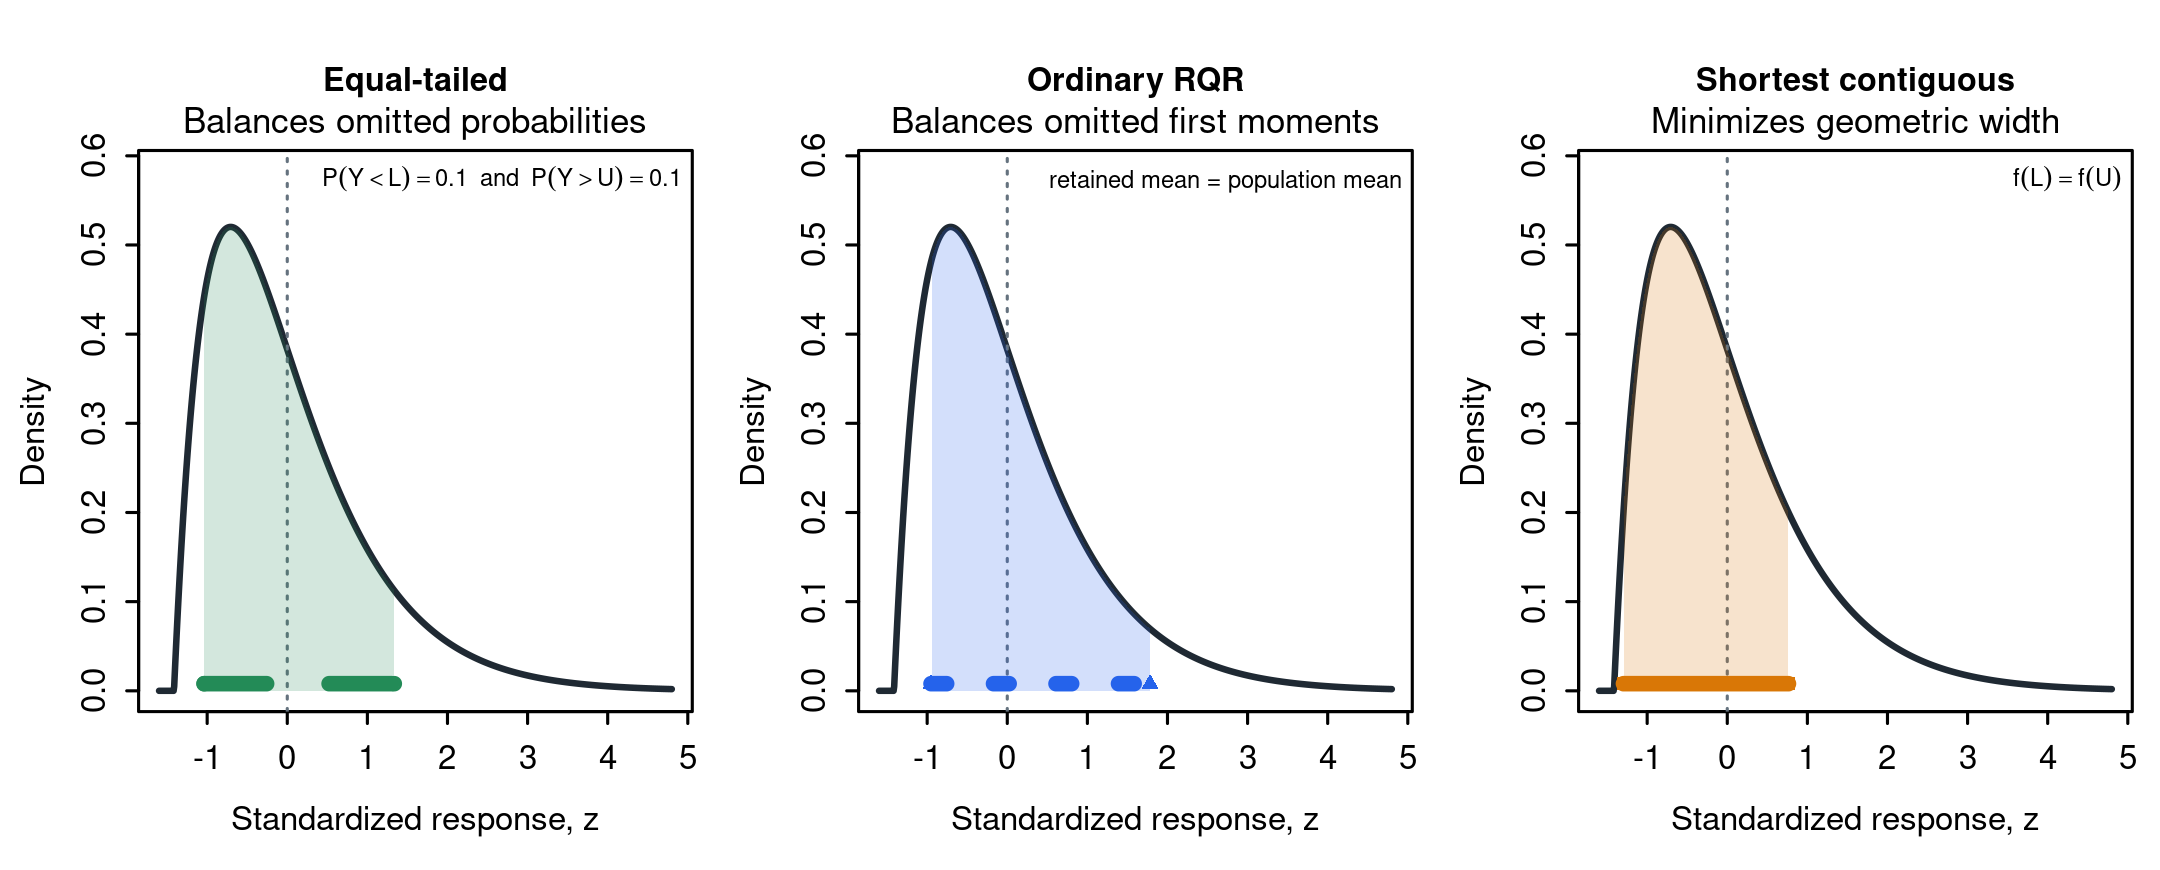
\includegraphics[width=\textwidth]{figures/generated/fig01_three_balance_principles.png}
\caption{\textbf{Three interval-selection principles under right skewness.}
All panels use a standardized \(\mathrm{Gamma}(2,1)\) population distribution
and content \(c=0.80\). Equal-tailed (ET) intervals balance omitted
probabilities, ordinary RQR balances omitted first moments, and shortest
contiguous (SH) intervals minimize geometric width. Color, line type, and
endpoint shape redundantly encode the three targets. These deterministic
population calculations compare the functionals; they do not provide
finite-sample or comparative-performance evidence.}
\label{fig:three-interval-principles}
\end{figure}

\section{Ordinary Relaxed Quantile Regression}
\label{sec:rqr-loss}

Let \(y_i\) be the response and let \(\vect x_i\in\R^p\) be a fixed design row,
for \(i=1,\ldots,n\). For a content level \(c\in(0,1)\), define two
exchangeable root readouts
\[
\eta_{1i}=\vect x_i^\top\vect\beta_1,\qquad
\eta_{2i}=\vect x_i^\top\vect\beta_2.
\]
The reported interval endpoints are ordered after fitting:
\[
L_i=\min(\eta_{1i},\eta_{2i}),\qquad
U_i=\max(\eta_{1i},\eta_{2i}).
\]
The root labels are not lower and upper labels; they are exchangeable
computational labels.

Define the residual product
\[
e_i=(y_i-\eta_{1i})(y_i-\eta_{2i})
\]
and the check loss
\[
\rho_c(e)=e\{c-\ind(e<0)\}.
\]
Then \(e_i<0\) if and only if \(y_i\) lies between the two roots. The empirical
RQR loss is
\[
\mathcal L_{n,c}(\vect\beta_1,\vect\beta_2)
=\sum_{i=1}^n \rho_c(e_i).
\]
For population interpretation, write the ordered endpoints as
\(a=m-h\) and \(b=m+h\), where \(h>0\). Then
\[
(Y-a)(Y-b)=(Y-m)^2-h^2.
\]
The half-width \(h\) controls interval content, while the midpoint \(m\)
controls which content-\(c\) interval is selected. The results below concern
an unrestricted pointwise population problem. Restricted regression classes
generally recover only design-weighted projections of these identities.

\begin{proposition}[Mean-preserving population target]
\label{prop:population-characterization}
Fix \(x\) and let \(a<b\). Suppose
\(\E(Y^2\mid X=x)<\infty\), the conditional distribution has no mass at \(a\)
or \(b\), differentiation may be interchanged with conditional expectation,
and \((a,b)\) is an interior stationary point over an unrestricted pointwise
endpoint class. Then the two population first-order conditions imply
\[
\Pr(a<Y<b\mid X=x)=c,
\]
and
\[
\E\{Y\ind(a<Y<b)\mid X=x\}
=c\,\E(Y\mid X=x).
\]
Equivalently,
\[
\E(Y\mid a<Y<b,X=x)=\E(Y\mid X=x).
\]
\end{proposition}

The population content implication is due to
\citet{PouplinEtAl2024RQR}. The conditional first-moment equation is a further
consequence of the same first-order system and does not appear in the original
RQR article. It is equivalently zero conditional covariance
between \(Y\) and interval membership. It also balances the first-moment
contributions removed from the two tails rather than their probabilities:
\[
\int_{-\infty}^{a}\{\mu_x-y\}\,dF_x(y)
=
\int_b^\infty\{y-\mu_x\}\,dF_x(y),
\qquad \mu_x=\E(Y\mid X=x).
\]
The retained core and its excluded complement consequently have the same
conditional mean, although the endpoint midpoint need not equal that mean.
The supplement further shows that the retained core is a mean-preserving
contraction of the full distribution in convex order. A finite first moment is
enough for the retained-mean identity once the endpoint scores are valid. The
stronger second-moment assumption ensures that the product-check risk is finite
and supports the profiled-risk analysis. This distinction matters because the
loss grows quadratically in an extreme response.

\begin{theorem}[Quantile-window identification]
\label{prop:quantile-window}
In addition to the conditions of
Proposition~\ref{prop:population-characterization}, suppose that \(F_x\) is
continuous and strictly increasing on its support, and let \(Q_x=F_x^{-1}\).
Define
\[
M_{c,x}(u)=\frac{1}{c}\int_u^{u+c}Q_x(v)\,dv,
\qquad 0\le u\le1-c.
\]
Then \(M_{c,x}\) is strictly increasing and there is a unique index \(u_c(x)\)
such that \(M_{c,x}\{u_c(x)\}=\mu_x\). The nondegenerate unrestricted RQR
stationary interval is therefore
\[
a_c(x)=Q_x\{u_c(x)\},\qquad
b_c(x)=Q_x\{u_c(x)+c\}.
\]
If \(F_x\) is symmetric about \(\mu_x\), then
\(u_c(x)=(1-c)/2\), and the RQR and equal-tailed intervals coincide.
\end{theorem}

This theorem identifies the unique regular stationary window.
Proposition~\ref{prop:profiled-mean-tilt} below strengthens that statement to
the unique global expected-loss minimizer by profiling over the half-width.
The supplement proves these results and records the restricted score
equations. As \(c\) varies, the regular unrestricted population intervals form
a nested path that contracts to the conditional mean as \(c\) decreases to
zero. This path statement does not turn the midpoint at a fixed positive
content into a mean estimator. If the conditional law has endpoint atoms,
the corresponding directional conditions give
\[
\Pr(a<Y<b\mid X=x)\le c\le\Pr(a\le Y\le b\mid X=x),
\]
so exact open-interval coverage requires endpoint continuity. Coincident roots
reduce the loss to \(c(Y-a)^2\) and target the conditional mean rather than a
nontrivial interval. Exact retained-mean equality is not asserted at endpoint
atoms without a separate joint subgradient and mass-allocation analysis.

This motivates RQR as a direct interval target that can adapt to asymmetric
conditional error structure without assigning endpoint quantile levels in
advance. These equations characterize an unrestricted population target only
under the stated conditions. With linear or otherwise restricted root classes,
optimization instead enforces design-weighted score equations; it need not
give conditional coverage or mean preservation at every covariate value. We do
not use the original article's finite-sample unbiasedness argument: fitted
endpoints are data dependent, and the empirical objective is nonsmooth when an
observation coincides with a root. A valid finite-sample or asymptotic
generalization result requires a separate empirical-process analysis.

\section{Mean-Tilted RQR}
\label{sec:mean-tilt}

To move through the content-\(c\) family without changing the coverage score,
consider a fixed mean tilt \(\delta\), measured in response units, and define
\[
\ell_{c,\delta}(m,h;y)
=
\rho_c\{(y-m)^2-h^2\}-2c\delta(m-y).
\]
Equivalently,
\[
\ell_{c,\delta}(a,b;y)
=
\rho_c\{(y-a)(y-b)\}-c\delta(a+b-2y).
\]
The second form shows that the loss remains invariant to exchanging the two
roots.

\begin{proposition}[Fixed-content mean tilt]
\label{prop:mean-tilt}
Under the regularity conditions of
Proposition~\ref{prop:population-characterization}, a nondegenerate interior
stationary point of the mean-tilted population risk satisfies
\[
\Pr(a_\delta<Y<b_\delta)=c,\qquad
\E(Y\mid a_\delta<Y<b_\delta)=\mu+\delta.
\]
If \(F\) is continuous and strictly increasing on its support, then for every
\(\delta\) strictly between \(M_c(0)-\mu\) and
\(M_c(1-c)-\mu\), its unique interior quantile-window index solves
\[
M_c(u_\delta)=\mu+\delta.
\]
\end{proposition}

\begin{theorem}[Profiled identification of the interior target]
\label{prop:profiled-mean-tilt}
Suppose that the support closure is an interval (possibly with infinite
endpoints), \(F\) is absolutely continuous and strictly increasing between its
support endpoints, its density is positive and continuous on the support
interior, and \(\E(Y^2)<\infty\). Extend \(F\) by zero and one beyond finite
support endpoints. Then, for every finite midpoint \(m\), there is a unique
radius \(h_c(m)>0\) satisfying
\(\Pr\{|Y-m|<h_c(m)\}=c\). Define the profiled risk
\[
\overline R_{c,\delta}(m)
=
\E\{\ell_{c,\delta}(m,h_c(m);Y)\}.
\]
Let \(u_c(m)=F\{m-h_c(m)\}\), with \(u_c(m)=0\) or \(1-c\) when the
corresponding root extends beyond a finite support endpoint. Then
\[
\overline R_{c,\delta}'(m)
=
2c\left[M_c\{u_c(m)\}-\mu-\delta\right]
\]
where the derivative exists, with the analogous one-sided statement at a
support transition. Consequently, for
\[
M_c(0)-\mu<\delta<M_c(1-c)-\mu,
\]
the expected mean-tilted loss has a unique global minimizer over finite ordered
roots. Its index \(u_\delta\in(0,1-c)\) is the unique solution of
\[
M_c(u_\delta)=\mu+\delta.
\]
Nondegeneracy gives \(M_c(0)<\mu<M_c(1-c)\), so ordinary RQR is the interior
special case \(\delta=0\). Exchanging the two raw root labels leaves the target
unchanged.
\end{theorem}

The supplement proves the radius existence and uniqueness, the envelope
derivative, and the one-sided behavior when an interval root crosses a finite
support endpoint. Finite second moments make both endpoint tilt values finite, even when a
support endpoint is infinite. At an endpoint tilt, the canonical interval is
defined by the corresponding one-sided probability-window limit. If the
support endpoint is infinite, this member is semi-infinite and is not attained
by finite root coefficients, although the limiting infimum is finite. If the
support endpoint is finite, roots beyond that endpoint are inactive and the
population loss does not identify a unique root representation without an
additional support constraint. Tilts outside the closed admissible range make
the unrestricted population risk unbounded below in the corresponding
escaping-root direction, although a proper Gaussian prior can still yield a
proper finite-sample generalized posterior.

\begin{corollary}[Recovery tilts for familiar interval functionals]
\label{cor:recovery-tilts}
Ordinary RQR is recovered by \(\delta_{\mathrm{RQR}}=0\). Define
\[
\mathcal U_{\mathrm{SH}}
=
\argmin_{0\le u\le1-c}W_c(u),\qquad
\Delta_{\mathrm{SH}}
=
\{M_c(u)-\mu:u\in\mathcal U_{\mathrm{SH}}\}.
\]
The population recovery tilt for the equal-tailed interval is
\[
\delta_{\mathrm{ET}}=M_c\{(1-c)/2\}-\mu.
\]
Each \(u\in\mathcal U_{\mathrm{SH}}\) has recovery tilt
\(\delta_{\mathrm{SH}}(u)=M_c(u)-\mu\). Singular notation is used only when the
shortest-contiguous window is unique or one minimizer has been selected.
\end{corollary}

For an interior tilt,
\[
\frac{du_\delta}{d\delta}=\frac{c}{W_c(u_\delta)},\qquad
\frac{dW_c(u_\delta)}{d\delta}
=\frac{c\,W_c'(u_\delta)}{W_c(u_\delta)}.
\]
Thus an interior width minimum along the tilt path satisfies the usual
equal-endpoint-density condition.
Figure~\ref{fig:mean-tilt-map} traces this one-to-one interior map and its
width profile for the same population benchmark.

\begin{figure}[h!]
\centering
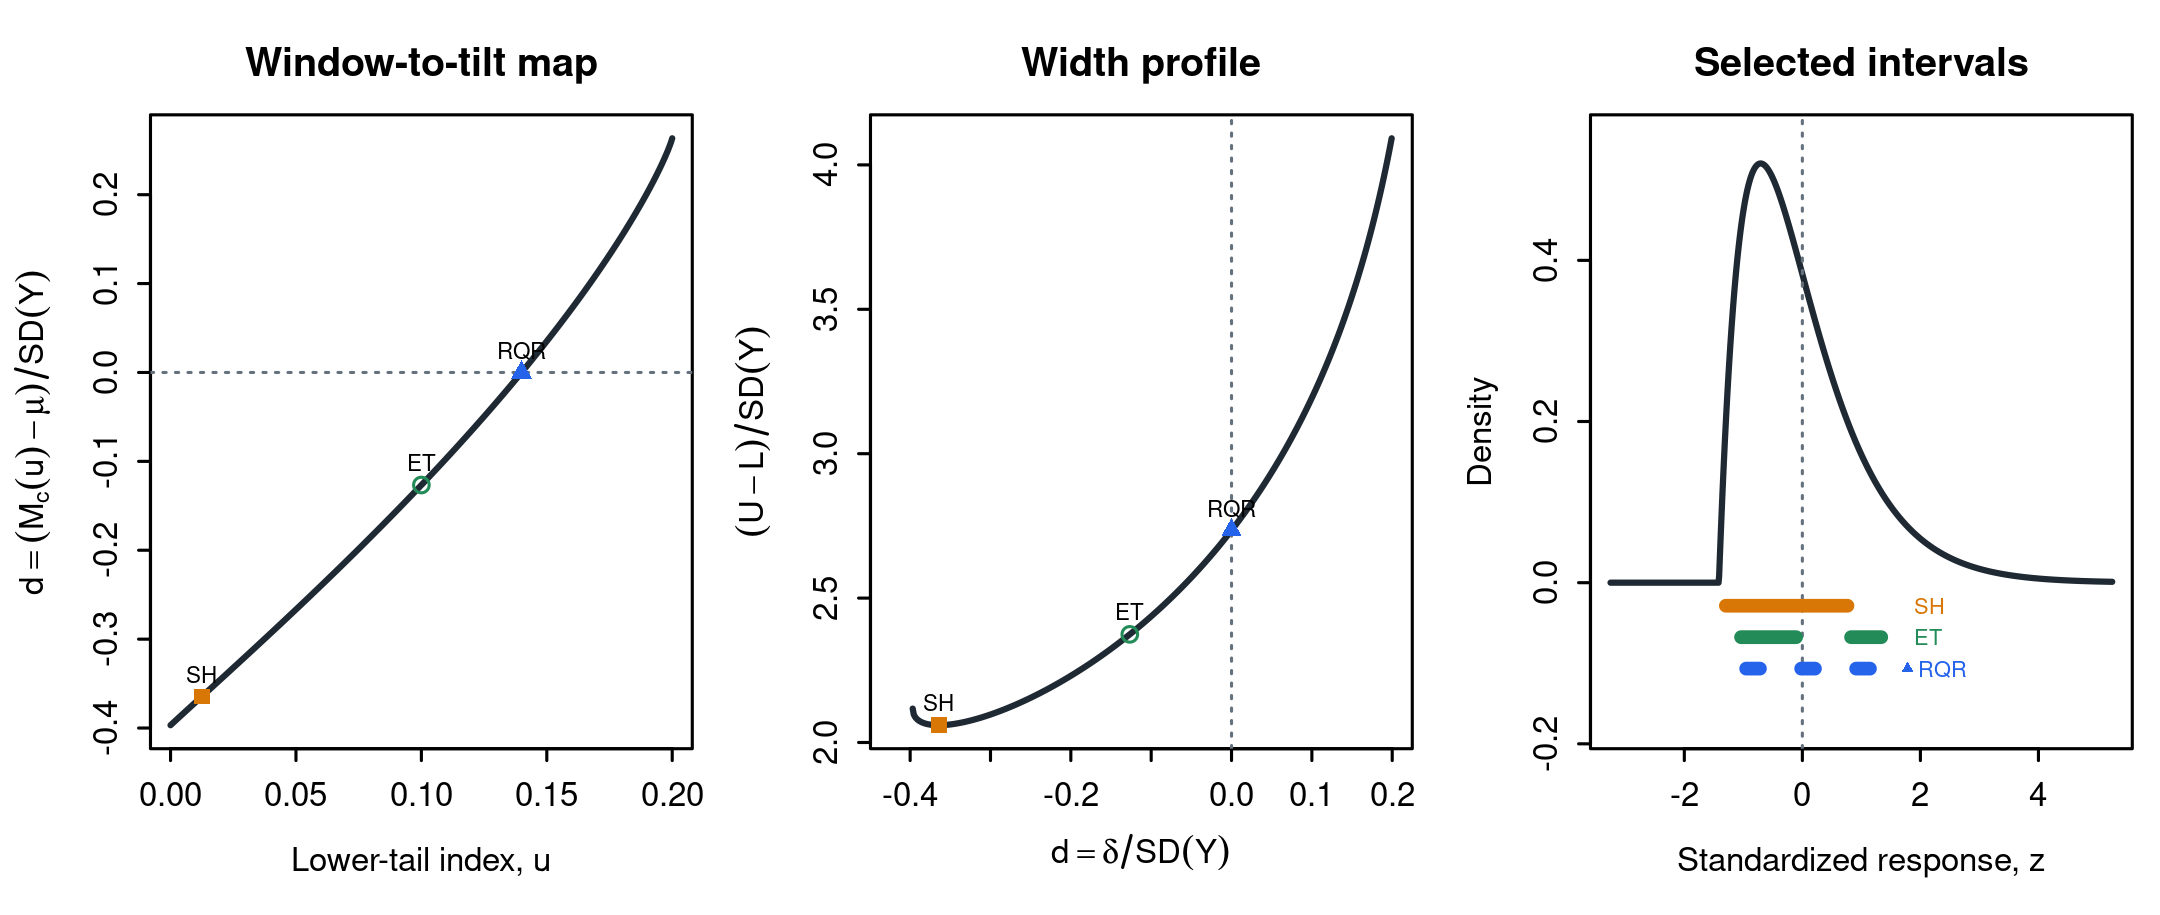
\includegraphics[width=\textwidth]{figures/generated/fig02_mean_tilt_recovery_map.png}
\caption{\textbf{Population mean-tilt recovery map.}
For a \(\mathrm{Gamma}(2,1)\) distribution and \(c=0.80\), the retained-window
mean \(M_c(u)\) maps each interior lower-tail index \(u\) to a unique
standardized tilt \(d=\delta/\operatorname{SD}(Y)\). The marked oracle tilts
recover the shortest contiguous (SH), equal-tailed (ET), and ordinary-RQR
intervals; ordinary RQR has \(d=0\). The width profile shows that SH, not
ordinary RQR in general, minimizes geometric width. The quantities are
deterministic population calculations describing representability and width
profiling; they do not define a data-driven tilt estimator.}
\label{fig:mean-tilt-map}
\end{figure}

These are population and oracle statements. A universal tilt does not recover
the same interval functional across distributions, and conditional recovery
generally requires a covariate-dependent \(\delta(x)\). The tilt should
initially be fixed or selected in an external training/validation layer;
sampling it as an ordinary parameter would mix distinct interval targets. The
target is equivariant under positive affine changes of response scale when
\(\delta\) and the fixed learning rate are transformed accordingly, but it is
not invariant to arbitrary monotone response transformations. The current
RQR-DLM implementation and validation protocol use \(\delta=0\). Mean-tilted
computation and data-driven tilt selection require their own code and
validation before empirical claims are made.

The population score equations do not by themselves establish propriety of a
finite-sample generalized posterior under an arbitrary root prior. For a fixed
learning rate, a finite design or finite state horizon, and proper Gaussian
root priors, the tilt is linear in the root parameters and Gaussian prior tails
make the tilted kernel integrable. This argument covers the initial ridge and
Gaussian-state implementations; heavier-tailed shrinkage priors require a
separate propriety analysis before nonzero tilt is enabled.

\section{Generalized Posterior and Gibbs Computation}
\label{sec:posterior}

\subsection{Declared loss targets and augmentation}

For priors \(\pi_\beta(\vect\beta_1)\) and
\(\pi_\beta(\vect\beta_2)\), define the generalized posterior
\[
\Pi_{\mathrm R}
(d\vect\beta_1,d\vect\beta_2\mid\vect y,\mat X)
\propto
\pi_\beta(d\vect\beta_1)\pi_\beta(d\vect\beta_2)
\exp\{-\omega_{\mathrm R}\mathcal L_{n,c}(\vect\beta_1,\vect\beta_2)\},
\]
where \(\omega_{\mathrm R}>0\) is a learning rate. A learned-scale version
uses a positive reference loss scale \(s_L\), sets
\(\omega_{\mathrm R}=\kappa/s_L\), and places a Gamma prior on \(\kappa\).
We call

\[
\Pi_{\mathrm R}(d\vartheta,d\kappa\mid\vect y)
\propto
\pi(d\vartheta)\kappa^{n}\pi_\kappa(d\kappa)
\exp\{-\kappa\mathcal L_{n,c}(\vartheta)/s_L\},
\]
the \emph{pseudo-residual-normalized learned-scale target}. The factor
\(\kappa^n\) arises from normalizing an asymmetric-Laplace kernel in the
abstract pseudo-residual \(e_i\); it does not normalize a response density in
\(y_i\). Here \(\vartheta\) collects both roots. If
\(\kappa\sim\mathrm{Gamma}(a_\kappa,b_\kappa)\) in shape--rate form, its
collapsed conditional is

\[
\kappa\mid\vartheta,\vect y
\sim\mathrm{Gamma}\left(a_\kappa+n,
b_\kappa+\mathcal L_{n,c}(\vartheta)/s_L\right).
\]
The factor \(\kappa^n\) is part of the declared target rather than an
irrelevant constant when \(\kappa\) is learned. A pure-loss sensitivity target
that omits this factor is kept separate.

The learned \(\kappa\) is part of this declared hierarchical generalized
target. Coherence for a fixed loss scale does not establish that \(\kappa\) is
an ordinary jointly learnable response parameter or that its generalized
posterior calibrates endpoint uncertainty
\citep{LeeLiuNicholls2025LearningRate,WuMartin2023LearningRateComparison}.
We therefore use fixed-rate sensitivity analyses as the primary specification
and treat learned-scale inference as an additional convention. When \(s_L\) is
computed from training responses, its calculation sample and variance
convention are recorded and \(s_L\) is frozen before simulation; the resulting
target is data dependent in an empirical-Bayes sense.

Let
\[
r_i=y_i^2,\qquad
m_i^{\mathrm R}=y_i(\eta_{1i}+\eta_{2i})-\eta_{1i}\eta_{2i}.
\]
Then \(r_i-m_i^{\mathrm R}=e_i\). With
\[
\sigma_{\mathrm R}=s_L/\kappa=\omega_{\mathrm R}^{-1},\qquad
\xi_c=\frac{1-2c}{c(1-c)},\qquad
\phi_c=\frac{2}{c(1-c)},
\]
the exponentiated loss contribution is proportional to
\[
\int_0^\infty
\Normal\!\left(
r_i\mid m_i^{\mathrm R}+\xi_c v_i,\,
\phi_c\sigma_{\mathrm R}v_i
\right)
\Exp(v_i\mid \text{rate}=1/\sigma_{\mathrm R})\,dv_i .
\]
This identity is a computational representation of the loss kernel. It should
not be read as a response model for \(y_i\).
Figure~\ref{fig:gibbs-computational-schematic} summarizes the resulting scan
without assigning a response-generating interpretation to the augmentation.

\begin{figure}[t]
\centering
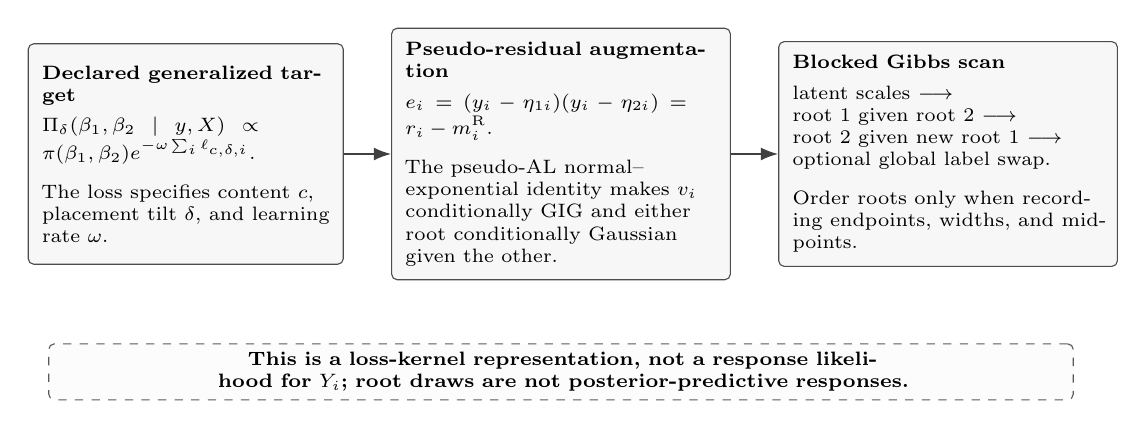
\begin{tikzpicture}[
  font=\scriptsize,
  >={Latex[length=2.2mm]},
  flow/.style={draw=black!70, rounded corners=2pt, fill=black!3,
    align=left, inner sep=5pt, minimum height=2.8cm},
  arrow/.style={->, semithick, black!75},
  warning/.style={draw=black!65, dashed, rounded corners=2pt,
    fill=black!1, align=center, inner sep=3pt}
]
  \node[flow, text width=3.65cm] (target) {
    \textbf{Declared generalized target}\par\smallskip
    \(\displaystyle
      \Pi_{\delta}(\beta_1,\beta_2\mid y,X)\propto
      \pi(\beta_1,\beta_2)
      e^{-\omega\sum_i\ell_{c,\delta,i}}.
    \)\par\medskip
    The loss specifies content \(c\), placement tilt \(\delta\),
    and learning rate \(\omega\).
  };

  \node[flow, text width=3.95cm, right=6mm of target] (augment) {
    \textbf{Pseudo-residual augmentation}\par\smallskip
    \(\displaystyle
      e_i=(y_i-\eta_{1i})(y_i-\eta_{2i})
      =r_i-m_i^{\mathrm R}.
    \)\par\medskip
    The pseudo-AL normal--exponential identity makes \(v_i\)
    conditionally GIG and either root conditionally Gaussian
    given the other.
  };

  \node[flow, text width=3.95cm, right=6mm of augment] (scan) {
    \textbf{Blocked Gibbs scan}\par\smallskip
    latent scales \(\longrightarrow\)\par
    root 1 given root 2 \(\longrightarrow\)\par
    root 2 given new root 1 \(\longrightarrow\)\par
    optional global label swap.\par\medskip
    Order roots only when recording endpoints, widths, and midpoints.
  };

  \draw[arrow] (target) -- (augment);
  \draw[arrow] (augment) -- (scan);

  \node[warning, text width=12.8cm, below=8mm of augment] (scope) {
    \textbf{This is a loss-kernel representation, not a response likelihood
    for \(Y_i\); root draws are not posterior-predictive responses.}
  };
\end{tikzpicture}

\caption{\textbf{Computational augmentation and Gibbs scan.}
The generalized posterior exponentiates a declared interval-root loss; it is
not a response-likelihood posterior. The pseudo-asymmetric-Laplace
normal--exponential representation gives GIG latent-scale updates and Gaussian
conditional updates for the exchangeable root blocks. Current software
implements ordinary RQR (\(\delta=0\)); the nonzero fixed-\(\delta\)
information shift is derived but not implemented or validated. Ordered
endpoints, widths, and midpoints are interval-root functionals, not
posterior-predictive response draws.}
\label{fig:gibbs-computational-schematic}
\end{figure}

\subsection{Conditional Gibbs blocks}
\label{sec:gibbs}

Conditional on \(\vect\beta_2\), the pseudo-observation equation is linear in
\(\vect\beta_1\):
\[
\mat A_1=\diag(\vect y-\vect\eta_2)\mat X,\qquad
\vect z_1=\vect y\circ(\vect y-\vect\eta_2)-\xi_c\vect v.
\]
With \(W_v=\diag\{(\phi_c\sigma_{\mathrm R}v_i)^{-1}\}\) and Gaussian prior
canonical parameters \((\mat Q_{01},\vect h_{01})\),
\[
\mat Q_1=\mat Q_{01}+\mat A_1^\top W_v\mat A_1,\qquad
\vect h_1=\vect h_{01}+\mat A_1^\top W_v\vect z_1,
\]
so
\[
\vect\beta_1\mid\cdot\sim
\Normal(\mat Q_1^{-1}\vect h_1,\mat Q_1^{-1}).
\]
The update for \(\vect\beta_2\) is identical after swapping root labels. The
latent scales have generalized inverse Gaussian full conditionals. For the
learned-scale target, one valid partially collapsed scan draws \(\kappa\) from
its collapsed Gamma conditional, refreshes all latent scales using that new
draw, and then updates roots 1 and 2. The refresh order is part of the sampler
contract. Adaptive shrinkage priors use separate shrinkage states for the two
root coefficient vectors.

\begin{algorithmblock}{Ordinary-RQR fixed-design Gibbs scan}
\label{alg:fixed-design-gibbs}
\item Initialize both root coefficient blocks, their prior or shrinkage
states, and---for the normalized learned-scale target---\(\kappa\).
\item If the learning rate is fixed, retain its declared value. If it is
learned, draw \(\kappa\) from the collapsed Gamma conditional using the
current roots, and set \(\sigma_{\mathrm R}=s_L/\kappa\).
\item Draw each \(v_i\) from its GIG full conditional using the current roots
and the current \(\sigma_{\mathrm R}\). In the learned-scale scan, this refresh
must follow the collapsed \(\kappa\) draw.
\item Draw \(\vect\beta_1\) conditional on \(\vect\beta_2\), then draw
\(\vect\beta_2\) conditional on the newly sampled \(\vect\beta_1\), using the
Gaussian systems above. Update any root-specific shrinkage states.
\item Optionally apply a global root-label swap. Record label-invariant
functionals through ordered endpoints \(L_i,U_i\), widths, and midpoints.
\end{algorithmblock}

For completeness, a scalar fixed mean tilt preserves these conditional
families. Under a fixed learning rate, the two Gaussian information vectors
become
\[
\vect h_k^{\mathrm{MT}}
=\vect h_k+\omega_{\mathrm R}c\delta\mat X^\top\vect 1_n,
\qquad k=1,2.
\]
The latent-scale conditional and Gaussian precision matrices are unchanged.
The supplement gives the algebraic covariate-specific vector extension. These
are fixed-rate identities, not evidence of an implemented nonzero-tilt API.
They do not extend the current learned-scale Gamma update: the tilted loss need
not be nonnegative, and a normalized joint target with random learning rate
must be derived separately.

\section{Dynamic RQR: A Root-State Model}
\label{sec:dynamic}

For an RQR-DLM or state-space embedding, each root can be represented by a
latent state path, for example
\[
\eta_{kt}=F_t^\top\theta_{kt},\qquad
\theta_{kt}=G_t\theta_{k,t-1}+\epsilon_{kt},
\qquad \epsilon_{kt}\sim\Normal(0,W_{kt}),
\qquad k=1,2.
\]
The two trajectories can be written as one stacked state with block-diagonal
evolution matrices. That representation does not, however, give one Gaussian
FFBS update. Jointly in the two root states, the augmented observation kernel
contains the square of
\[
(y_t-F_t^\top\theta_{1t})(y_t-F_t^\top\theta_{2t}),
\]
and therefore includes fourth-order cross-terms. Conditional on either complete
root path, the same expression is linear in the other path. The sampler
accordingly partitions the stacked state by root and uses two sequential FFBS
blocks. These are exact full-conditional updates for the declared fixed-joint
target; the issue is potential Markov-chain mixing, not posterior
approximation.

Conditional on the second root path and the RQR latent scales, the first root
path enters through
\[
z_{1t}=y_t(y_t-\eta_{2t})-\xi_c v_t,\qquad
H_{1t}=(y_t-\eta_{2t})F_t^\top,qquad
V_t=\phi_c s_Lv_t/\kappa.
\]
This is a scalar-observation Gaussian state-space system, so the complete root
path can be sampled by forward-filtering backward-sampling. The second root
path is analogous and conditions on the newly drawn first path.

The evolution specification matters to the target. Fixed \(W_{kt}\) defines a
Gaussian state prior and gives exact alternating FFBS. A frozen discount
template first maps component-specific discounts to a complete \(W_{1:T}\)
sequence through a declared reference covariance recursion and then holds that
sequence fixed throughout MCMC. Conditional on that template, this gives an
exact sampler for the stated prior; a template estimated from training data is
recorded as an empirical-Bayes specification. By contrast, recomputing \(W_t\)
from each conditional filter covariance
makes it depend on the other root and latent-scale blocks. We retain that
exdqlm-compatible recursion only as an experimental working update. A
two-time scalar mixed-derivative argument in the supplement shows that its two
advertised conditional FFBS kernels are generally incompatible with a common
positive smooth joint density.

For an exact component-specific alternative, partition the state into blocks
and set
\[
W_t(\vect q)=\operatorname{blockdiag}
\{q_1Q_{1t},\ldots,q_JQ_{Jt}\},
\qquad q_j\sim\operatorname{IG}(a_j,b_j),
\]
where \(Q_{jt}\) are fixed positive-definite templates. The multipliers are
shared across the two roots to preserve prior exchangeability. Sampling the
time-zero states restores the innovation factorization and yields conjugate
inverse-Gamma updates for each \(q_j\); the complete derivation appears in the
supplement.

\begin{algorithmblock}{Ordinary-RQR root-blocked dynamic Gibbs scan}
\label{alg:dynamic-gibbs}
\item Initialize both complete state paths, \(v_{1:T}\), any shared component
scales, and---for the normalized learned-scale target---\(\kappa\).
\item If \(\kappa\) is learned, draw it from its collapsed Gamma conditional
using both current root paths. Then refresh every \(v_t\) from its GIG
conditional. For a fixed learning rate, begin with the same latent-scale
refresh at the declared rate.
\item Conditional on \(\theta_{2,1:T}\), sample
\(\theta_{1,0:T}\) by FFBS from its scalar-observation Gaussian state-space
full conditional.
\item Conditional on the newly sampled \(\theta_{1,1:T}\), sample
\(\theta_{2,0:T}\) by the analogous FFBS update.
\item For a shared component-scale model, update each \(q_j\) from its
inverse-Gamma full conditional using innovations from both roots, including
the sampled time-zero states.
\item Optionally swap the two complete root paths. Retain ordered endpoint,
width, midpoint, state, scale, and loss summaries.
\end{algorithmblock}

Algorithm~\ref{alg:dynamic-gibbs} applies only to ordinary RQR and the declared
fixed-joint evolution modes. A fixed nonzero tilt would add a known
time-varying information shift to each conditional FFBS block, but neither
that sampler nor a learned-scale tilted target is implemented here.

\section{Evaluation Strategy and Evidence Scope}
\label{sec:evaluation}

The evaluation separates population identities, sampler validation, and
comparative forecasting evidence. Deterministic population calculations test
the fixed-content and mean-tilt characterizations without Monte Carlo error.
Small reference problems compare Gibbs output with quadrature, dense Gaussian
conditionals, analytic scale updates, and exact checkpoint continuation. These
checks establish target and implementation agreement for the stated fixtures;
they do not establish empirical coverage calibration or forecasting
superiority.

The matched ordinary-RQR study uses common data-generating mechanisms,
training and forecast windows, content levels, seeds, and scoring rules across
fixed-design RQR, RQR-DLM, separately fitted quantile intervals, and empirical
baselines. Primary summaries are held-out RQR loss, empirical coverage error,
width at comparable coverage, and endpoint recovery when a population oracle
is available. The equal-tailed interval score is secondary because it targets
a different placement principle. Dynamic diagnostics use time-local and
future ordered roots, widths, midpoints, losses, learning scales, and
component scales rather than only time averages.

Current computational evidence concerns ordinary RQR. Nonzero mean tilt
requires zero-tilt equivalence checks, independent small-target references,
and fixed-design validation at prespecified population tilts before any
data-driven selection rule is evaluated. Variational inference likewise
requires its own target, derivation, and uncertainty assessment. A
deterministic-feature RQR-DESN readout remains a secondary extension: its
reservoir is a recorded design object, while the generalized posterior updates
only the root readouts. Detailed software status, runtime attestation, and
validation ledgers belong to the reproducibility documentation rather than to
the statistical argument.

\section{Discussion}
\label{sec:discussion}

Probability content alone determines a class, not an interval placement.
Ordinary RQR selects its mean-preserving member under the stated population
conditions. The mean tilt exposes the larger geometry: each admissible
interior value specifies a retained mean and hence one contiguous
content-\(c\) window. Equal-tailed and shortest-contiguous intervals are
distribution-specific members of this family rather than universally named
tilt values.

This interpretation also clarifies the role of Bayesian computation. The
normal--exponential representation is an augmentation of an exponentiated
loss in a pseudo-residual. It makes the root blocks conditionally Gaussian,
but it neither supplies a response likelihood nor licenses simulated
responses. The learned inverse-loss scale \(\kappa\) is a convention within a
declared normalized generalized target, not a response variance or an
automatic endpoint-calibration parameter.

The dynamic extension preserves the same interval target while allowing its
roots to evolve. A Gaussian stacked prior does not overcome the quartic joint
observation term; exact computation instead alternates the two Gaussian
root-path conditionals. Fixed evolution covariances, frozen discount
templates, and shared component scales define fixed-joint targets. Recomputing
discount covariances from each changing conditional filter remains a working
recursion, not an exact Gibbs sampler for a demonstrated joint density.

Important limitations remain. The population results are unrestricted and
pointwise, whereas fitted regression and state-space classes impose
projections. Boundary tilts can yield semi-infinite limits or inactive roots,
and tilts outside the admissible range have no finite unrestricted target.
Nonzero-tilt algorithms, external tilt selection, variational approximations,
and matched nonlinear-readout evidence require separate validation. The
ordinary-RQR study is therefore designed to evaluate interval-root loss,
empirical coverage, width, and endpoint recovery without conflating any of
them with posterior-predictive response calibration.

\bibliographystyle{plainnat}
\bibliography{refs}

\end{document}
